% Rapport à éditer directement. Les figures sont produites par les scripts.
\documentclass[10pt,a4paper]{article}
\usepackage[T1]{fontenc}
\usepackage[utf8]{inputenc}
\usepackage[french]{babel}
\usepackage{lmodern,amsmath,booktabs,tabularx,float,caption,xcolor,graphicx,hyperref,fancyhdr}
\usepackage[margin=17mm,headheight=13pt]{geometry}
\definecolor{bluecol}{HTML}{315E73}\definecolor{redcol}{HTML}{AE483E}\definecolor{graycol}{HTML}{AAAAAA}
\hypersetup{colorlinks=true,urlcolor=bluecol,linkcolor=bluecol,citecolor=bluecol}
\setlength{\parindent}{0pt}\setlength{\parskip}{4pt}
\setlength{\textfloatsep}{7pt}\setlength{\intextsep}{6pt}
\captionsetup{font=footnotesize,skip=3pt}
\renewcommand{\arraystretch}{1.12}
\pagestyle{fancy}\fancyhf{}\fancyfoot[L]{\footnotesize Soudures -- apprentissage automatique}\fancyfoot[R]{\footnotesize\thepage}
\renewcommand{\headrulewidth}{0pt}\renewcommand{\footrulewidth}{0pt}
% Informations du binôme.
\newcommand{\Etudiants}{Hiyu SHINTANI -- \href{mailto:hiyu.shintani@student-cs.fr}{hiyu.shintani@student-cs.fr}\\Anas LECAILLON -- \href{mailto:anas.lecaillon@student-cs.fr}{anas.lecaillon@student-cs.fr}}
\newcommand{\DateRapport}{12 octobre 2026}
\graphicspath{{output/figures/}}
\begin{document}

{\Large\bfseries\color{bluecol}Prédiction d'un niveau de résistance à la traction des soudures}\par

\textbf{Projet d'apprentissage automatique -- CentraleSupélec, 3A}\\\DateRapport{}\\\Etudiants{}

\textbf{Plan :} problématique et données ; prétraitement, ACP et validation ; méthodes ; résultats ; discussion et conclusion.

\section{Problématique et données}

Le projet cherche à prédire la qualité de soudures d'acier et à identifier les paramètres associés à de bonnes propriétés. La base ne contient pas d'étiquette universelle de qualité : résistance, ductilité et ténacité mesurent des dimensions différentes. Nous retenons une cible simple, la résistance à la traction, sans confondre une résistance élevée avec une qualification industrielle complète.

La tâche est une \textbf{classification binaire} : $y=1$ si la résistance mesurée est supérieure ou égale à la médiane des valeurs connues de l'apprentissage, et $y=0$ sinon. Le seuil est recalculé dans chaque pli, sans les réponses de validation, puis figé sur le développement pour le test final. Il est relatif au jeu de données, sans valeur normative. Une cible manquante reste inconnue ; elle n'est jamais imputée comme un vrai label.

\subsection{Base publique et choix des variables}

La base MAP\_DATA\_WELD\cite{data} contient 1652 observations et 44 colonnes : 738 résistances à la traction connues et 914 absentes. Les mesures connues vont de 447 à 1151 MPa. La figure~\ref{fig:data} décrit les valeurs absentes et la distribution de la cible.

Les \textbf{colonnes 1 à 30} sont les entrées : composition (pourcentage massique ou ppm), intensité (A), tension (V), apport thermique (kJ/mm), températures (${}^\circ$C), durée (h), courant, polarité et procédé de soudage. Les propriétés mécaniques et la microstructure, colonnes 31 à 43, sont exclues des prédicteurs pour éviter de prédire un résultat à partir d'autres résultats postérieurs à la fabrication. L'identifiant sert uniquement au groupement.

\begin{figure}[H]
\centering
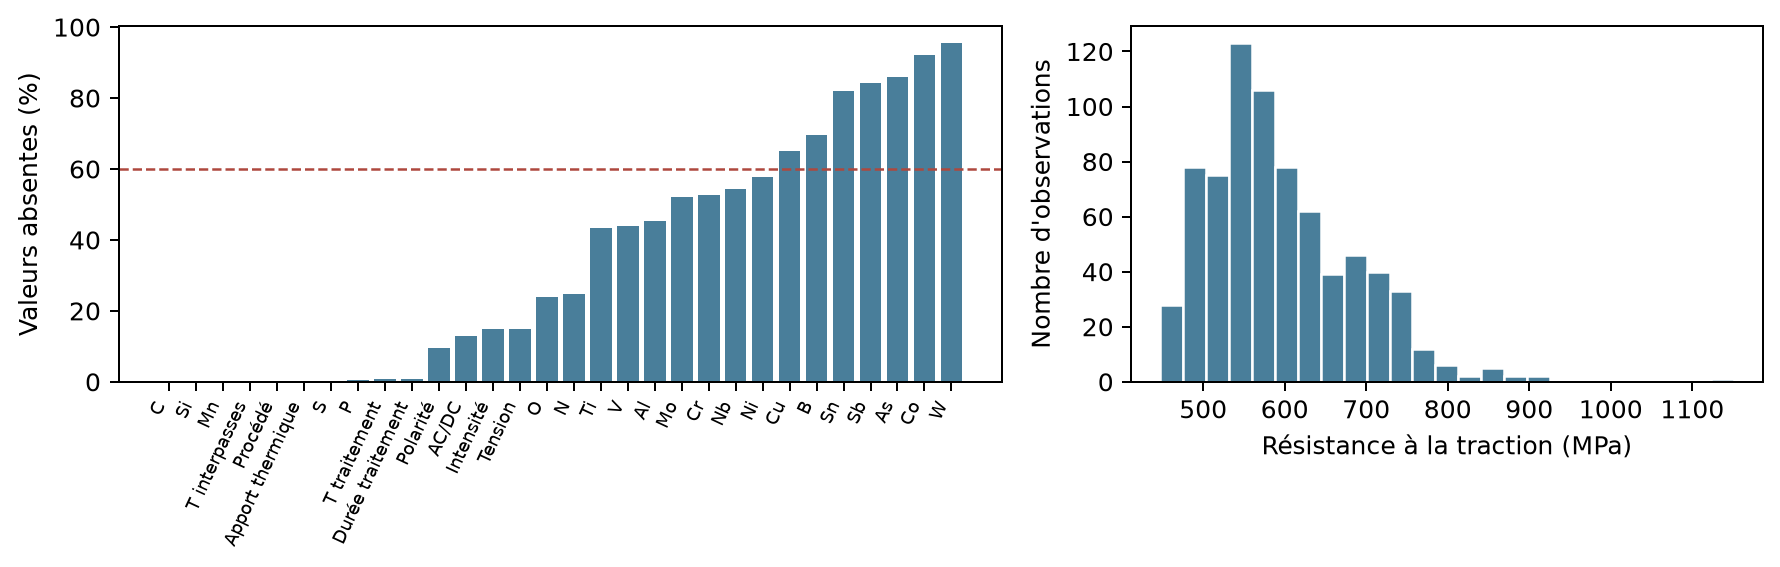
\includegraphics[width=.98\linewidth,height=4.8cm,keepaspectratio]{data_overview.png}
\caption{Absence des entrées et distribution de la résistance à la traction. La ligne pointillée indique le seuil pratique de filtrage à 60\%.}\label{fig:data}
\end{figure}

La description et les unités des 44 variables sont exportées dans un dictionnaire. Les valeurs extrêmes ne sont pas supprimées automatiquement : une composition rare peut représenter un cas réel plutôt qu'une erreur.

\clearpage

\section{Prétraitement, ACP et validation}

La documentation distingue \texttt{N} (non renseigné) de zéro. Les formats spéciaux sont audités : $<x$ devient $x/2$, approximation au milieu de $[0,x]$ ; la température 150--200 est remplacée par 175~${}^\circ$C ; pour l'azote \texttt{tot...res}, seule la valeur totale est retenue. Les annotations de dureté Hv sont conservées dans l'audit, mais cette variable reste exclue des modèles. Les limites de détection ne sont pas transformées en mesures exactes. Une analyse de sensibilité compare ensuite $x/2$ à 0 et à $x$.

\begin{table}[H]\centering\small
\begin{tabularx}{\linewidth}{p{.30\linewidth}X}
\toprule
\textbf{Traitement} & \textbf{Justification} \\
\midrule
Entrée constante ou >60 \% manquante : retrait & Limiter les entrées essentiellement imputées ; convention pratique, apprise dans chaque pli. \\
Médiane numérique & Conserver les lignes incomplètes ; réduire la sensibilité aux extrêmes. \\
Catégorie manquant et one-hot & Ne pas inventer d'ordre entre les modalités ; accepter les modalités nouvelles. \\
Centrage-réduction pour ACP et k-NN & Rendre les échelles comparables ; inutile pour les arbres. \\
\bottomrule
\end{tabularx}
\caption{Préparation des entrées, ajustée uniquement sur l'apprentissage.}\label{tab:prep}
\end{table}

Les traitements du tableau~\ref{tab:prep} sont ajustés sans la validation ni le test. Les populations avec et sans cible diffèrent : médiane du chrome renseigné 0,05\% contre 2,07\%, et température de traitement médiane 250 contre 0~${}^\circ$C. Ces écarts limitent la représentativité des observations non labélisées.

\subsection{ACP exploratoire}

L'ACP utilise 20 entrées numériques, imputées et centrées-réduites, sur 1329 observations de développement, avec ou sans cible. PC1 explique 18,9\% de la variance et PC2 14,7\% ; 10 composantes atteignent 80\%. La projection de la figure~\ref{fig:pca} présente un recouvrement des classes. L'ACP cherche à préserver la variance des entrées, sans chercher directement la meilleure discrimination.

\begin{figure}[H]
\centering
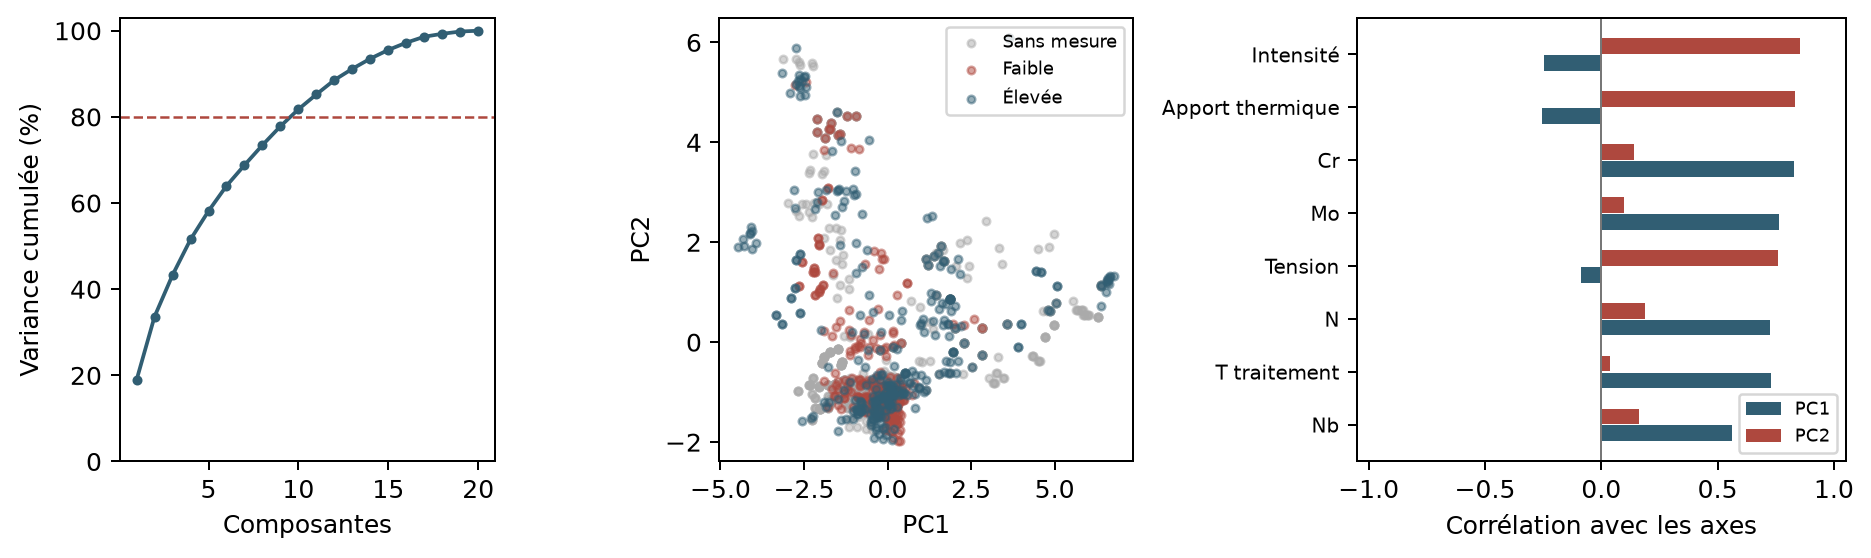
\includegraphics[width=.98\linewidth,height=4.0cm,keepaspectratio]{pca.png}
\caption{Variance expliquée, projection des observations et corrélations avec les axes. Les couleurs distinguent les classes et les mesures absentes.}\label{fig:pca}
\end{figure}

Les principales corrélations avec PC1 concernent Cr, Mo, pwht\_temperature, N ; avec PC2, current, heat\_input, voltage, S. Chaque composante combine plusieurs variables. L'ACP développe l'intuition ; les modèles utilisent les entrées préparées directement.

\subsection{Séparation par groupes}

Identifiants répétés, variantes de suffixes et profils de fabrication identiques sont réunis en 651 groupes conservateurs. Avec la graine 42, le développement contient 1329 lignes (520 groupes) et le test 323 lignes (131 groupes). Une validation croisée à cinq plis par groupes évite qu'un groupe se retrouve des deux côtés. Les lignes non labélisées de validation ou de test restent aussi hors apprentissage semi-supervisé. Cette heuristique ne garantit pas l'indépendance de toutes les publications d'origine.

\clearpage

\section{Méthodes et protocole expérimental}

Nous comparons une référence majoritaire à trois approches complémentaires : k-NN pour la prédiction par proximité, CART pour des règles lisibles et une forêt aléatoire pour combiner des arbres et limiter leur variance. Une forêt peut néanmoins mal généraliser à une autre population. Les petites grilles du tableau~\ref{tab:grid} limitent le coût de recherche.

\begin{table}[H]\centering\small
\begin{tabularx}{\linewidth}{p{.22\linewidth}X}
\toprule
\textbf{Modèle} & \textbf{Réglages comparés} \\
\midrule
Majoritaire & Classe la plus fréquente de l'apprentissage ; aucun réglage. \\
k-NN & k = 3, 5, 11, 21 ; distance euclidienne après normalisation. \\
Arbre CART & Profondeur 3, 5, 10 ; minimum 5 ou 10 observations par feuille. \\
Forêt aléatoire & 200 arbres ; profondeur 5, 10 ou libre ; minimum 2 ou 5 par feuille ; max\_features = sqrt. \\
\bottomrule
\end{tabularx}
\caption{Familles de modèles et recherche d'hyperparamètres limitée.}\label{tab:grid}
\end{table}

Le critère de sélection est le F1 macro moyen en validation croisée. À moins de 0,01 du meilleur score, nous préférons le réglage le plus simple : profondeur réduite, feuilles plus grandes ou k plus grand. Entre familles, l'ordre de préférence est arbre, k-NN, forêt. Les scores CV sont des scores de sélection ; le test, utilisé après fixation des choix, apporte l'évaluation indépendante.

\subsection{Self-training avec la forêt}

Le self-training réutilise la forêt sélectionnée plutôt que d'ajouter une nouvelle famille de modèles. Un premier modèle apprend les labels connus ; ses prédictions les plus confiantes sur les entrées inconnues deviennent des pseudo-labels, puis le modèle est réentraîné. La revue bibliographique souligne qu'une erreur initiale peut s'auto-renforcer et que l'utilisation de données sans label ne garantit pas une amélioration\cite{zhu}.

L'implémentation retient les pseudo-labels dont la probabilité maximale est \textbf{strictement supérieure à 0,90}, avec arrêt après dix itérations ou sans nouvel ajout\cite{sklearn}. Ce seuil est une convention de sélection, pas une probabilité garantie de justesse : les probabilités de la forêt ne sont pas calibrées dans cette étude.

Pour isoler l'effet des pseudo-labels, le prétraitement des deux forêts est appris sur les mêmes entrées labélisées visibles puis appliqué aux entrées inconnues de l'apprentissage. Les labels d'origine ne sont jamais remplacés. L'hypothèse est que la proximité et les premières prédictions confiantes correspondent suffisamment bien aux classes ; une frontière artificielle à la médiane et des données hétérogènes peuvent la fragiliser.

\subsection{Expériences de raréfaction des labels}

Nous comparons la forêt et le self-training avec les mêmes labels disponibles : 100\%, puis 25\% et 50\% conservés uniformément avec les graines 42, 43 et 44. Seuls les labels visibles fixent le seuil ; la validation reste labélisée. Les réponses masquées permettent un contrôle a posteriori des pseudo-labels, sans intervenir dans les réglages. Les seuils changent entre fractions et graines : il faut comparer les deux méthodes au sein d'un même essai. Cette simulation n'isole pas un effet de quantité de labels sur une cible fixe.

\subsection{Métriques}

Pour chaque classe, considérée tour à tour comme positive :\[P=\frac{TP}{TP+FP},\qquad R=\frac{TP}{TP+FN},\qquad F_1=\frac{2TP}{2TP+FP+FN}.\]$TP$, $FP$ et $FN$ désignent les vrais positifs, faux positifs et faux négatifs. Le \textbf{F1 macro} est la moyenne non pondérée des deux F1 ; l'accuracy est la proportion totale de bonnes prédictions. Une division indéfinie vaut zéro. Moyennes et écarts-types sont descriptifs, sans être des intervalles de confiance : les plis et essais partagent des données.

\clearpage

\section{Résultats numériques}

\begin{table}[H]\centering\small
\begin{tabularx}{\linewidth}{lccX}
\toprule
\textbf{Modèle} & \textbf{F1 macro CV} & \textbf{Accuracy CV} & \textbf{Réglage retenu} \\
\midrule
Majoritaire & 0,348 \ensuremath{\pm} 0,027 & 0,535 & Aucun \\
k-NN & 0,799 \ensuremath{\pm} 0,033 & 0,802 & k = 5 \\
Arbre CART & 0,751 \ensuremath{\pm} 0,022 & 0,761 & Profondeur 3 ; feuille 5 \\
Forêt aléatoire & 0,838 \ensuremath{\pm} 0,028 & 0,841 & Profondeur 10 ; feuille 2 \\
\bottomrule
\end{tabularx}
\caption{Moyenne et écart-type des plis pour chaque réglage choisi.}\label{tab:cv}
\end{table}

La sélection du tableau~\ref{tab:cv} retient Forêt aléatoire. Le tableau~\ref{tab:test} évalue les modèles sur 145 vrais labels de test : 68 faibles et 77 élevés, avec un seuil figé à 575,0 MPa.

\begin{table}[H]\centering\small
\begin{tabularx}{\linewidth}{Xcccc}
\toprule
\textbf{Test final} & \textbf{F1 macro} & \textbf{Accuracy} & \textbf{Rappel faible} & \textbf{Rappel élevé} \\
\midrule
Majoritaire & 0,347 & 0,531 & 0,000 & 1,000 \\
Forêt aléatoire & 0,862 & 0,862 & 0,926 & 0,805 \\
Self-training & 0,869 & 0,869 & 0,956 & 0,792 \\
\bottomrule
\end{tabularx}
\caption{Performance sur les groupes de test réservés avant la sélection.}\label{tab:test}
\end{table}

\begin{figure}[H]
\centering
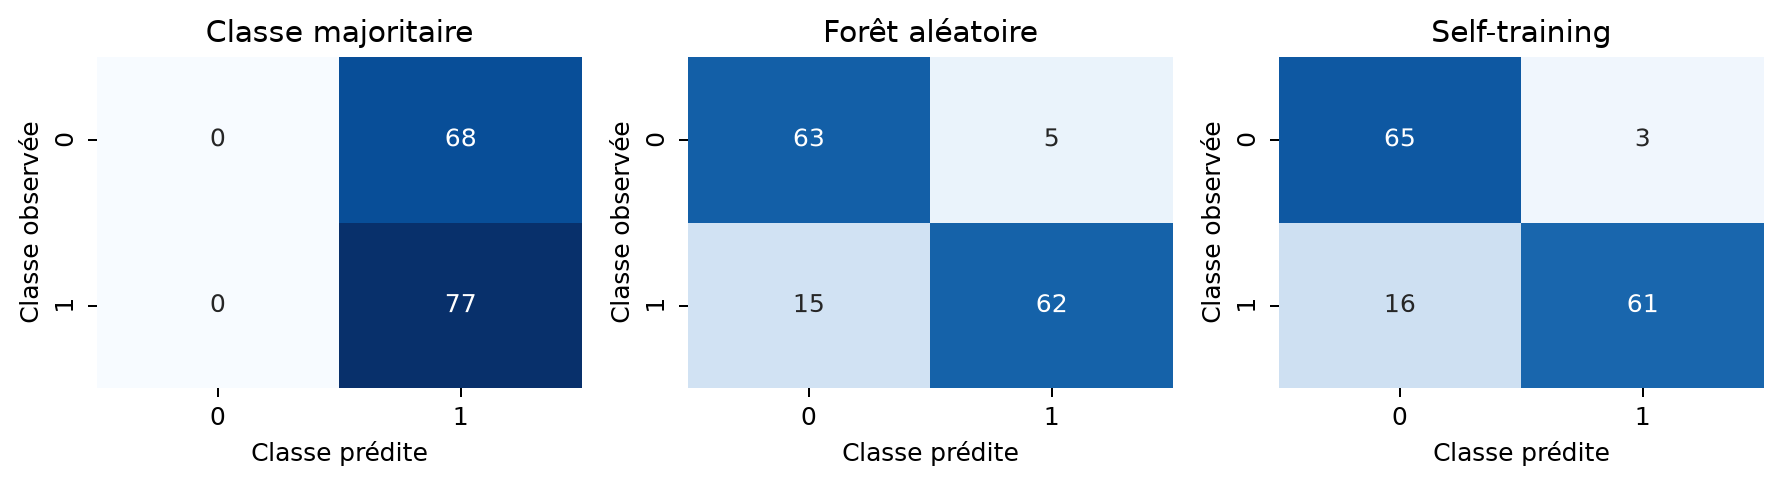
\includegraphics[width=.98\linewidth,height=3.1cm,keepaspectratio]{confusion.png}
\caption{Matrices de confusion du test : classes 0 (faible) et 1 (élevée). Les lignes sont les observations, les colonnes les prédictions.}\label{fig:confusion}
\end{figure}

\begin{figure}[H]
\centering
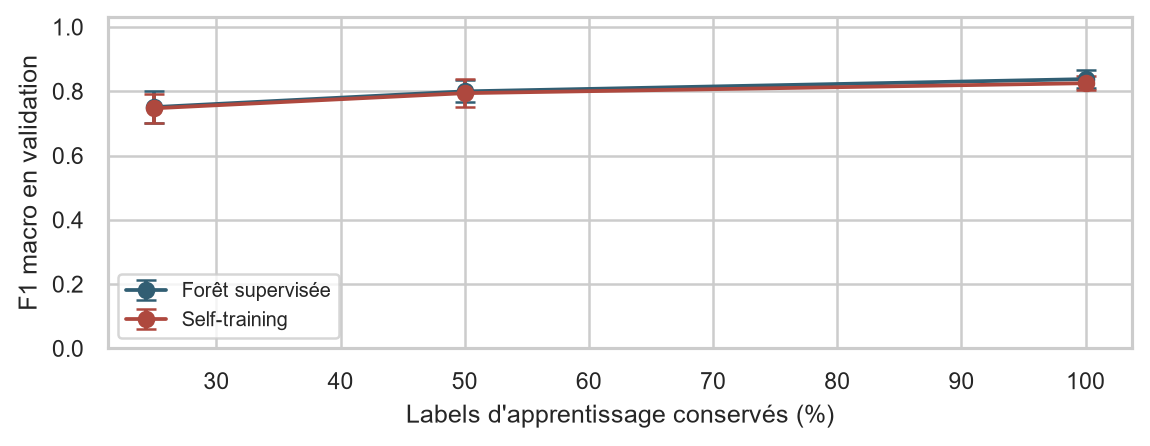
\includegraphics[width=.98\linewidth,height=4.1cm,keepaspectratio]{semi_supervised.png}
\caption{Validation des deux forêts aux mêmes labels visibles. Barres : écart-type entre plis et, à 25/50\%, graines de masquage.}\label{fig:ssl}
\end{figure}

À 100\% des labels disponibles, le self-training modifie le F1 CV moyen de -0,013 par rapport à la forêt (figure~\ref{fig:ssl}). Dans les masquages, 2983 pseudo-labels acceptés ont une vérité connue, avec 93,8\% de justesse agrégée. Les mêmes observations peuvent être comptées dans plusieurs essais ; la vérité des mesures naturellement absentes reste inaccessible.

Sur le modèle supervisé retenu, la convention de censure change peu le F1 CV moyen : $x/2$ = 0,838, borne $x$ = 0,839, zéro = 0,837. La convention initiale $x/2$ est maintenue ; aucune convention n'est choisie à partir du test.

\clearpage

\section{Discussion et conclusion}

\begin{table}[H]\centering\small
\begin{tabularx}{\linewidth}{lX}
\toprule
\textbf{Entrée} & \textbf{Baisse de F1 par permutation (moyenne \ensuremath{\pm} écart-type)} \\
\midrule
Mn & 0,063 \ensuremath{\pm} 0,017 \\
Cr & 0,052 \ensuremath{\pm} 0,018 \\
Nb & 0,045 \ensuremath{\pm} 0,019 \\
Mo & 0,036 \ensuremath{\pm} 0,018 \\
O & 0,013 \ensuremath{\pm} 0,008 \\
\bottomrule
\end{tabularx}
\caption{Importance de la forêt : cinq permutations par entrée, sur chaque validation.}\label{tab:importance}
\end{table}

Les variables les plus utiles (tableau~\ref{tab:importance}) sont Mn, Cr, Nb. Elles décrivent une utilité prédictive, pas une causalité. Les variables corrélées peuvent partager ou masquer leur importance. Dans le développement, la traction médiane est 611,5 MPa dans la tranche de Mn la plus haute, contre 560,5 dans la plus basse ; pour Cr, 699,0 contre 570,15 MPa. Ces populations diffèrent aussi sur d'autres facteurs.

\textbf{Recommandations.} Examiner avec un expert matériaux les compromis associés au manganèse, au chrome et au niobium, sans maximiser un élément isolément ; comparer les réglages dans des conditions comparables et vérifier expérimentalement les associations ; mesurer aussi allongement et ténacité avant de qualifier une soudure ; enrichir les mesures manquantes et clarifier les unités et limites de détection.

\textbf{Conclusion.} La forêt reste le choix principal, sélectionné avant le test, avec F1 macro = 0,862. Le self-training classe correctement une observation supplémentaire sur ce test, mais il est moins bon en moyenne en CV. Ses résultats sont mitigés. Les limites sont le seuil non normatif, les réponses manquantes potentiellement sélectives, les approximations de préparation et les dépendances entre études. Le test ne valide ni une nouvelle population industrielle ni une optimisation causale.

\begingroup\footnotesize\setlength{\parskip}{1pt}\begin{thebibliography}{9}

\bibitem{data} T. Cool et H. K. D. H. Bhadeshia. \emph{MAP\_DATA\_WELD}, University of Cambridge. \href{https://www.phase-trans.msm.cam.ac.uk/map/data/materials/welddb-b.html}{Documentation des données}.

\bibitem{zhu} X. Zhu. \emph{Semi-Supervised Learning Literature Survey}, TR 1530, University of Wisconsin--Madison, version du 19 juillet 2008, sections 1 et 3. \href{https://pages.cs.wisc.edu/~jerryzhu/pub/ssl_survey.pdf}{Rapport technique}.

\bibitem{sklearn} scikit-learn. \emph{Semi-supervised learning}, section Self Training : seuil de confiance, itérations et probabilités fiables. \href{https://scikit-learn.org/stable/modules/semi_supervised.html}{Documentation}. Consultée le 12/10/2026.

\end{thebibliography}\endgroup\end{document}

